\documentclass[a4paper,12pt,twoside]{scrreprt}
% nezbytné balíčky
\usepackage[T1]{fontenc}
\usepackage[utf8]{inputenc}  % vstupní znaková sada: UTF8
\usepackage[czech]{babel} % typografická pravidla     
\usepackage[a4paper, hmarginratio=3:2]{geometry} % využití celé A4 stránky a nastavení okrajů
\usepackage{graphicx} % balíček pro vkládání obrázků
\usepackage{tabularx} % rozšířené možnosti tabulek
\usepackage{indentfirst}
\usepackage{titlesec} 

% balíčky, které se mohou hodit
%\usepackage{amsmath} % balíček pro pokročilou matem. sazbu
%\usepackage{color} % pro možnost barevného textu
%\usepackage{fancybox} % umožňuje pokročilé rámečkování
%\usepackage{index} % nutno použít v případě tvorby rejstříku balíčkem makeindex
%\newindex{default}{idx}{ind}{Rejstřík} % zavádí rejstřík v případě použití balíku index
%\usepackage{caption} % pro popisky obrázků, tabulek atd.
%\usepackage{listings}  % balíček vhodný pro ukázky kódu 
%\usepackage{float} % rozšířené možnosti umístění obrázků
%\usepackage[hidelinks]{hyperref} % pro klikací odkazy v pdf
%\usepackage{encxvlna} % postará se o spojky a předložky, které dle českých pravidel nesmí být na konci řádku. Dokumentace: http://texdoc.net/texmf-dist/doc/generic/encxvlna/encxvlna.pdf


% spacing: how to read {12pt plus 4pt minus 2pt}
%           12pt is what we would like the spacing to be
%           plus 4pt means that TeX can stretch it by at most 4pt
%           minus 2pt means that TeX can shrink it by at most 2pt
%       This is one example of the concept of, 'glue', in TeX
%		\titlespacing{command}{left spacing}{before spacing}{after spacing}[right]

\titlespacing{\section}{0pt}{\parskip}{-\parskip}
\titlespacing{\subsection}{0pt}{\parskip}{\parskip}
%\titlespacing{\subsubsection}{0pt}{\parskip}{-\parskip}

%\titlespacing\chapter{0pt}{0pt plus 2pt minus 2pt}{0pt plus 0pt minus 0pt}
%\titlespacing\section{0pt}{0pt plus 0pt minus 0pt}{0pt plus 0pt minus 0pt}
%\titlespacing\subsection{0pt}{2pt plus 4pt minus 2pt}{0pt plus 0pt minus 0pt}
%\titlespacing\subsubsection{0pt}{12pt plus 4pt minus 2pt}{0pt plus 2pt minus 2pt}

\topmargin=-15mm      % horní okraj trochu menší
\textwidth=150mm      % šířka textu na stránce
\textheight=240mm     % "výška" textu na stránce

\pagenumbering{arabic} % číslování stránek arabskými číslicemi
\pagestyle{plain}      % stránky číslované dole uprostřed

\parindent=22pt % odsazení 1. řádku odstavce
\parskip=7pt   % mezera mezi odstavci
\frenchspacing % aktivuje použití některých českých typografických pravidel

\newcommand{\ti}{\textit} %zkrácený příkaz pro kurzívu
\newcommand{\tb}{\textbf} %zkrácený příkaz pro tučné


%%%%%%%%%%%%%%%%%%%%%% zde jsou zavedeny některé "konstanty" - můžete, resp. musíte je ZMĚNIT %%%%%%%%%%%%%%%%%%%%%%
\newcommand{\cvut}{České vysoké učení technické v Praze}
\newcommand{\fjfi}{Fakulta jaderná a fyzikálně inženýrská}
\newcommand{\kse}{Katedra softwarového inženýrství v ekonomii}
\newcommand{\obor}{Inženýrská informatika}
\newcommand{\zamereni}{Softwarové inženýrství v ekonomii}

\newcommand{\nazevcz}{Modely zátěže výpočetních serverů}        % zde VYPLŇTE český název práce (přesně podle zadání!)
\newcommand{\nazeven}{Computational requirements modelling}     % zde VYPLŇTE anglický název práce (přesně podle zadání!)
\newcommand{\autor}{Dmitriy Burdin}           % zde VYPLŇTE své jméno a příjmení
\newcommand{\rok}{Červenec 2015}          % zde VYPLŇTE měsíc a rok odevzdání, např. May 2011
\newcommand{\vedouci}{Ing. Jan Doubek}         % zde VYPLŇTE jméno a příjmení vedoucího práce, včetně titulů, např. Doc. Ing. Ivo Malý, Ph.D.

\newcommand{\druh}{BAKALÁŘSKÁ PRÁCE}

\newcommand{\pracovisteVed}{CISCO Systems s.r.o.}			% zde VYPLŇTE pracoviště vedoucího práce

\newcommand{\konzultant}{-} % POKUD MÁTE určeného konzultanta, NAPIŠTE jeho jméno a příjmení
\newcommand{\pracovisteKonz}{-} % POKUD MÁTE konzultanta, NAPIŠTE jeho pracoviště


\newcommand{\klicova}{Časová řada, ekonometrie, predikce, analýza, server}   % zde NAPIŠTE česky max. 5 klíčových slov
\newcommand{\keyword}{Times series, econometrics, forecasting, analysis, server}       % zde NAPIŠTE anglicky max. 5 klíčových slov (přeložte z češtiny)
\newcommand{\abstrCZ}{Cílem této práce je efektivně modelovat časovou, výpočetní a paměťovou náročnost distribuovaných úloh. Implementace modelů na základě časových řad výsledků minulých úloh. Výsledkem práce bude studie použitelnosti ekonometrických metod v prostředí velkých data center. Dále návrh algoritmů pro implementaci studovaných metod. Výstupní modely budou použity pro lepší plánování rozvržení výpočetních zdrojů.} % zde NAPIŠTE abstrakt v češtině
\newcommand{\abstrEN}{The goal of this thesis is to effectively make a model of temporal, computational and memory requirements of distributed tasks. Model implementation based on time series results of past tasks. The result of the thesis will be a study of applicability of econometric methods in large scale data centres. In addition, design of algorithms for implementation of the studied methods. Output models will be used for better planning of computational sources arrangement.}                  % zde NAPIŠTE abstrakt v angličtině

\begin{document}

%%%%%%%%%%%%%%%%%%%%%% Titulní strana -- na následujících 30 řádků NESAHEJTE!!!  Generuje se AUTOMATICKY %%%%%%%%%%%%%%%%%%%%%%
\thispagestyle{empty}

\begin{center}
    {\Large \textsc{\cvut}\\[1.5ex] \textsc{\fjfi}}\\
    \vspace{10mm}

    \begin{tabular}{c}
	    {\bf \kse}\\   
      {\bf Obor: \obor}\\
      {\bf Zaměření: \zamereni}\\
    \end{tabular}

   % logo CVUT -- pokud jej nechcete použít, zakomentujte následující řádek a odkomentujte řádek pod ním:
   \vspace{10mm} 
\includegraphics[height=25mm]{lev.pdf} \vspace{15mm}
   % \vspace{50mm}

   {\huge \bf \nazevcz}\\
   \vspace{5mm}   
   {\huge \bf \nazeven}
   
   \vspace{15mm}
   {\Large \druh}

   \vfill
   {\large
    \begin{tabular}{ll}
    Vypracoval: & \autor\\
    Vedoucí práce: & \vedouci\\
    Rok: & \rok
    \end{tabular}
   }
\end{center}

%%%%%%%%%%%%%%%%%%%%%% Zadání práce  %%%%%%%%%%%%%%%%%%%%%%
%%%%%%%%%%%%%%%%%%%%%%            Před svázáním namísto této strany VLOŽÍTE zadání podepsané děkanem!
\newpage  % SEM NESAHEJTE!
\thispagestyle{empty} % SEM NESAHEJTE!

Před svázáním místo téhle stránky \fbox{vložíte zadání práce} s podpisem
děkana a do pdf verze oskenované zadání.

%oskenované zadání lze vložit jako obrázek

% 1. strana zadání
%\begin{center}
%     \includegraphics[width=1\textwidth]{zadani1.jpg}
%\end{center}

% 2. strana zadání
%\newpage  % SEM NESAHEJTE!
%\thispagestyle{empty} % SEM NESAHEJTE!
%\begin{center}
%     \includegraphics[width=1\textwidth]{zadani2.jpg}
%\end{center}

%%%%%%%%%%%%%%%%%%%%%% Prohlášení -- ŽENY UPRAVÍ minulý čas sloves %%%%%%%%%%%%%%%%%%%%%%
\newpage % SEM NESAHEJTE!
\thispagestyle{empty}  % SEM NESAHEJTE!

~ % SEM NESAHEJTE!
\vfill % prázdné místo. SEM NESAHEJTE!

{\bf Prohlášení} % SEM NESAHEJTE!

\vspace{0.5cm} % vertikální mezera. SEM NESAHEJTE!
Prohlašuji, že jsem svou bakalářskou práci vypracoval samostatně a použil jsem pouze podklady
(literaturu, projekty, SW atd.) uvedené v přiloženém seznamu.

\vspace{5mm}  % SEM NESAHEJTE!
\begin{tabularx}{\textwidth}{X c}                               	% SEM NESAHEJTE!
    V Praze dne .................... &........................................ \\	% SEM NESAHEJTE!
	& \autor
\end{tabularx}	% SEM NESAHEJTE!

%%%%%%%%%%%%%%%%%%%%%% Poděkování -- UPRAVTE JMÉNO, resp. tuto stránku celou VYMAŽTE %%%%%%%%%%%%%%%%%%%%%%
%%%%%%%%%%%%%%%%%%%%%%                           (poděkování nemusí být uvedeno vůbec)
\newpage
\thispagestyle{empty}

~
\vfill % prázdné místo

{\bf Poděkování}

\vspace{5mm} % vertikální mezera
Děkuji Ing. Janu Doubkovi za vedení mé bakalářské práce a za podnětné návrhy, které ji obohatily.

\begin{flushright}
\autor
\end{flushright}  % <------- tady končí stránka s poděkováním

%%%%%%%%%%%%%%%%%%%%%% Abstrakt atp. Je generován AUTOMATICKY podle údajů na začátku souboru) %%%%%%%%%%%%%%%%%
\newpage   % SEM NESAHEJTE!
\thispagestyle{empty}   % SEM NESAHEJTE!

% příprava:    (na následujících 8 řádků NESAHEJTE!)
\newbox\odstavecbox
\newlength\vyskaodstavce
\newcommand\odstavec[2]{%
    \setbox\odstavecbox=\hbox{%
         \parbox[t]{#1}{#2\vrule width 0pt depth 4pt}}%
    \global\vyskaodstavce=\dp\odstavecbox
    \box\odstavecbox}
\newcommand{\delka}{120mm} % šířka textů ve 2. sloupci tabulky

% použití přípravy:    % dovnitř "tabular" vůbec NESAHEJTE!
\begin{tabular}{ll}
  {\em Název práce:} & ~ \\
  \multicolumn{2}{l}{\odstavec{\textwidth}{\bf \nazevcz}} \\[0.5em]
  {\em Autor:} & \autor \\[0.5em]
  {\em Obor:} & \obor \\[0.5em]
  {\em Druh práce:} & \druh \\[0.5em]
  {\em Vedoucí práce:} & \odstavec{\delka}{\vedouci \\ \pracovisteVed} \\[0.5em]
  %{\em Konzultant:} & \odstavec{\delka}{\konzultant \\ \pracovisteKonz} \\[0.5em] % ZAKOMENTUJTE v případě, že jste neměli konzultanta
 \\[0.01em]  
  \multicolumn{2}{l}{\odstavec{\textwidth}{{\em Abstrakt:} ~ \abstrCZ  }} \\[0.5em]
 \\[0.01em]
  {\em Klíčová slova:} & \odstavec{\delka}{\klicova} \\[2em]

  {\em Title:} & ~\\
  \multicolumn{2}{l}{\odstavec{\textwidth}{\bf \nazeven}}\\[0.5em]
  {\em Author:} & \autor \\[0.5em]
  \multicolumn{2}{l}{\odstavec{\textwidth}{{\em Abstract:} ~ \abstrEN  }} \\[0.5em]
 \\[0.1em]
  {\em Key words:} & \odstavec{\delka}{\keyword}
\end{tabular}



%%%%%%%%%%%%%%%%%%%%%% Obsah práce ... je generován AUTOMATICKY %%%%%%%%%%%%%%%%%%%%%%
\newpage  % SEM NESAHEJTE!
\tableofcontents % SEM NESAHEJTE!


%%%%%%%%%%%%%%%%%%%%%%  Zde začíná SAMOTNÁ PRÁCE  %%%%%%%%%%%%%%%%%%%%%%%%%%%%%%%%%%%%%%%%%%%%
\newpage % SEM NESAHEJTE!

\chapter*{Úvod}
\addcontentsline{toc}{chapter}{Úvod} % SEM NESAHEJTE! 

Obrovské a rostoucí množství informací zaplavují dnešní podniky. To se stavá hlavně kvůli rostoucímu počtu lidí, firem a zařízení připojených k internetu. Kolem třetiny světové populace má dnes přístup k internetu. Velké množství informace, jinak řečeno - velká data, představuje rychle rostoucí sféru, ve které se pro maximální efektivitu vyžaduje vhodná kombinace softwaru, hardwaru a navíc speciální úpravy s ohledem na oblast působnosti. Tyto fakty vedou k výraznému zaměření na velká data a na nové metody správy a analýzování tohoto proudu informací. 

Důležitým prvkem řešení této problematiky je datacentrum. Jsou to specializované prostory pro umístění a zajištění stabilního provozu výpočetní a serverové techniky. Většinou se tato technika skládá z počítačových clusterů, což je několik spolupracujícich počítačů propojených počítačovou sítí. Clustery se využívají pro výpočet komplikovaných početních úloh. Jeden z hlavních parametrů kvalitních datacenter je správné planování distribuovaných úloh pro rychlé zpracování dat. Při stále se zvětšujícím množstvím dat se tento problém komplikuje. Proto je potřeba vědět v jakém pořadí zpracovávat určité úlohy a jak dlouho to bude trvat. 

Cílem této bakalářské práce bylo navrhnout a vytvořit softwarovou aplikaci pro analytické zpracování dat, se kterými pracjuí výpočetní servery. Podstatou aplikace je predikce budoucího chování určitých hodnont na základě analýzy minulých výsledků. Protože velká data obvykle obsahují dynamické systémy dat, které se mění s časem, zkoumaná data se předpokládají být ve formě časových řad. Proto se v této práci nejdřív věnuje způsobům zpracování, analýzy a predikce časových řad. Poté následjue popis algoritmu používání vybraných postupů pro vhodnou analýzu a implementace příslušného algoritmu. Na závěr je demonstrováno využítí aplikace na příkladových datech. 


\chapter{Teoretická část}

\section{Časové řady}
\subsection{Úvod a charakteristika}
Jak již bylo zmíněno, časové řady jsou základním zkoumaným prvkem při analýze různých dynamických systémů obsahující chronologicky uspořádaná data. Časové řady jsou vlastně soubory jednoznačně uspořádáných podle času pozorování v příslušném systému. Data ve formě časových řad vznikají v úplně různých odvětvích bud' to fyzikální věda, biologie, společenská věda, medicína atd. 

Například ve společenských vědách, časové řady jsou užitečné při popsání počtu obyvatel, porodnosti, nemocnosti. V ekonomii teorie časových řad je jednou z nejdůležitějších metod při analýze ekonomických procesů. Mohou popisovat vývoj určitého ukazatele jako objem výroby, produktivita práce, nezaměstnanost nebo spotřeba surovin. V technice časové řady mohou představovat průběh signálu, spolehlivost nebo intenzitu zatížení elektrického zařízení. 

Pro lepší porozumění určitého mechanismu nebo procesu, popsaného časovou řadou, existuje analýza časových řad skládající se z různých metod. Tyto metody pomáhají vytvořit vhodný model popisující chování pozorovaných hodnot. Znalost takového modelu umožňuje kontrolovat činnost a sledovat vývoj určitého systému. Jako důsledek spravné provedené analýzy stavá se možným predikovat budoucí chování systému.

Časové řady se skládají ze dvou prvků:
\begin{itemize}
\item časový úsek, během kterého byly udělány pozorování
\item hodnoty příslušných ukazatelů časové řady
\end{itemize}

Podle časového úseku časové řady se člení do dvou typů. Jedním je okamžiková časová řada, jejíž pozorování jsou naměřena v jisté časové okamžiky a sčítání hodnot příslušných pozorování nedává smysl. Příkladem může být řada udávající počet zaměstnanců ve firmě na začátku roku. Druhým typem je intervalová časová řada. Pozorování v intervalových časových řadách jsou závislé na délce časového intervalu sledování a v tomto případě už sčítání hodnot ukazatele časové řady dává smysl, nebot' hodnotu ukazatele za větší interval lze získat sčítáním hodnot za jednotlivé části příslušného intervalu. Například porodnost ve státě za rok. 

Časové úseky jsou obvykle stejnoměrně rozděleny, což znamená, že mezi jednotlivými pozorování stejné časové intervaly. V opačném případě pozorování jsou rozděleny různorodě a tím se analýza časových řad komplikuje. 

Obvykle rozlišujeme dva základní modely časových řad:
\begin{itemize}
\item Determenistický - model, ve kterém časová řada nemá náhodné prvky a je generována známou matematickou funkcí. Důsledkem je srovnatelně jednoduchá analýza časové řady. 
\item Stochastický - model popisuje náhodný proces a časová řada obsahuje náhodný prvek. Většina běžně se vyskytujících časových řad v praxi mají stochastické modely.
\end{itemize}

Jedna z dalších důležitých charakteristik časových řad, vyplývající ze stochastického modelu, je jejich stacionarita, případně nestacionarita. Při stacionaritě střední hodnota a rozptyl časové řady se v čase nemění, což nelze říct o nestacionárních časových řadách, ve kterých se objevují změny ve střední hodnotě či rozptylu. Říká se proto, že nestacionární časové řady mají určitý trend vývoje. I když stacionarita je běžným předpokladem většiny metod analýzy časových řad, některé modely se omezují na modely stacionárních procesů.  

\subsection{Analýza časových řad}
\normalsize \textbf{Grafická analýza časových řad}

Jedním ze základních prostředků prezentace časových řad je jejich graf. Nejčastěji
se graficky znázorňují původní hodnoty časové řady, nebo kumulativní časové řady, které
vznikají postupným načítáním (kumulováním) jednotlivých hodnot (u okamžikových
časových řad nemají smysl, neboť výše jejich hodnot nezávisí na daném časovém
intervalu). Často se ale časové řady zobrazují tak, aby více vynikly jejich charakteristické vlastnosti a rysy. K tomu slouží speciální typy grafů jako jsou například spojnicové grafy jedné nebo více časových řad, krabičkové grafy, grafy sezónních hodnot. 

Prvotní informace pro analýzu časových řad získáme ze \textbf{spojnicových grafů}. Jejich
princip spočívá v zakreslení jednotlivých hodnot časové řady do souřadných os, na kterých
jsou vyznačeny příslušné stupnice. Na osu horizontální se vynáší časová proměnná a na
osu vertikální hodnoty časové řady nebo její funkce.

Do spojnicového grafu můžeme zakreslit i více časových řad. V případě, že
zobrazujeme např. dvě časové řady lišící se měřítkem, je možné použít kromě levé 
i pravou vertikální osu.

V některých případech je užitečné provést detailnější pohled na časovou řadu.
\textit{Krabičkový graf} na rozdíl od jiných grafů obsahuje souhrnné charakteristiky zkoumané
časové řady. Tento graf umožní odhalit některé důležité vlastnosti řady, které z jiných
grafů nejsou zřetelné. Jeho základním prvkem je krabička, jejíž dolní a horní hrana je
tvořena 25\% a 75\% kvartilem, uvnitř je vyznačen medián a symbolem „+“ aritmetický
průměr. Na koncích svislých čar vycházejících z krabičky leží hodnoty minima a maxima.
Protože délka této svislé čáry může být maximálně 1,5x delší než krabička, jsou hodnoty
přesahující tyto hranice označovány jako odlehlé a jsou zakresleny jako samostatné body.

\begin{figure}
  \centering
  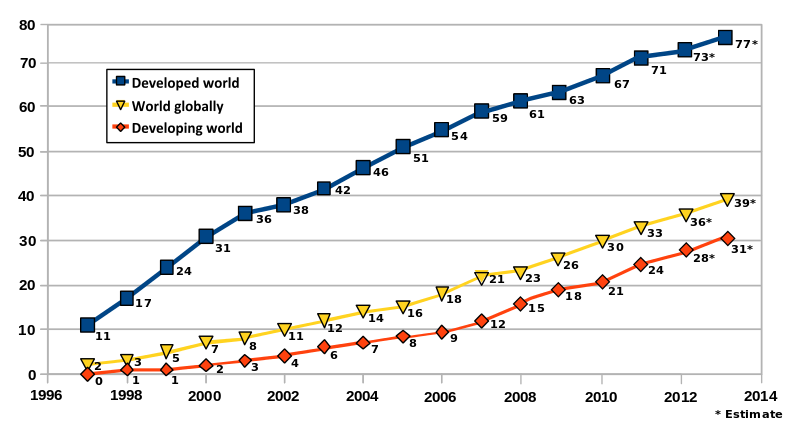
\includegraphics[width=15cm]{pictures/users.png}
  \caption{Počet uživatelů Internetu na 100 obyvatel ve světě. \newline(Příklad spojnicového grafu se třemi časovými řadami)}
  \label{fig:řada}
\end{figure}

\normalsize\textbf{\newline Dekompozice časových řad}

Abychom mohli s řadou pracovat, ve smyslu něco předpovídat, dělat odhady (ať už intervalové
či bodové) apod., potřebujeme mít alespoň stacionární časovou řadu. Respektivě alespoň slabě
stacionární časovou řadu. 

Většina pozorovaných časových řad není řadou nezávislých stejně rozdělených náhodných
veličin ani stacionární časovou řadou. Ale mnoho kdy se nám může podařit vhodným očistěním
řady, získat stacionární řadu. Eliminace jednotlivých složek časové řady, která se při dekompozici provádí, může mít různé cíle:

\begin{enumerate}
\item Zajímavé poznatky může přinést samotné studium oddělených (eliminovaných) složek časové řady, nebot' tak lze objevit některé zákonitosti chování sledované řady, rozpoznat vnější vlivy působící na její průběh a provést účinné srovnání průběhu několika časových řad. Např. pomocí trendové složky lze posuzovat tempo rozvoje dvou přibuzných průmzslových odvětví nebo pomocí sezónní složky lze posoudit průběh poptávky po určitém druhu zboží během roku. 
\item Podle bodu 1 je úkolem dekompozice časové řady proniknout hlouběji do podstaty historického průběhu řady. Neméně důležitým cílem dekompozice je ale také cíl extrapolační, kdy nás zajímá budoucí vývoj jednotlivých složek časové řady (např. jaké bude budoucí tempo růstu letecké přepravy) a nebo konstruujeme předpověd' v celé časové řadě tak, že ji složíme z předpovědí v jednotlivých složkách, které se obvykle sestrojí poměrně jednoduše a přesně. 
\item Často je vzhledem k podstatě řešeného problému výhodné znát chování časové řady "očištěné" od některých jejich složek. V ekonomických časových řadách se například velice často provádí tzv. sezónní očišťování, kdy z řady odstraňjeme sezónní fluktuace. 
\end{enumerate}

Klasická analýza ekonomických časových řad vychází z předpokladu, že časovou
řadu $y_t$ pro t = 1, 2, ... , T je možné rozložit na čtyři složky: trendovou, cyklickou, sezónní a nesystematickou.

\textit{Trendová složka} ($T_t$) vyjadřuje dlouhodobou tendenci vývoje zkoumaného jevu. Je výsledkem faktorů, které dlouhodobě působí stejným směrem např. technologie výroby, demografické podmínky, podmínky na trhu apod.

\textit{Cyklická složka} ($C_t$) vyjadřuje kolísání okolo trendu, ve kterém se střídají fáze růstu a poklesu. Jednotlivé cykly (periody) se vytvářejí za období delší než jeden rok a mají nepravidelný charakter, tj. různou délku a amplitudu. Cykly jsou v ekonomických časových řadách způsobeny ekonomickými a neekonomickými faktory. V posledních letech se věnuje pozornost zejména technologickým, inovačním či demografickým cyklům.

\textit{Sezónní složka} ($S_t$) vyjadřuje pravidelné kolísání okolo trendu v rámci kalendářního roku. Sezónní výkyvy se opakují každoročně ve stejných obdobích (délka periody je jeden rok) a vznikají v důsledku střídání ročních období nebo vlivem různých institucionalizovaných zvyků, jako jsou např. svátky, dovolené apod.

Poslední složkou časové řady je \textit{nesystematická složka} ($I_t$ nebo $a_t$). Tato složka vyjadřuje nahodilé a jiné nesystematické výkyvy, ale také chyby měření apod. 

Dekompozice časové řady může být:

\begin{enumerate}

\item aditivní, hodnoty časové řady se dají určit jako součet hodnot jednotlivých složek, tj.
\begin{equation}
y_t = T_t + C_t + S_t + I_t
\end{equation}

\item multiplikativní, hodnoty časové řady se dají určit jako součin hodnot jednotlivých složek
\begin{equation}
y_t = T_t \cdot C_t \cdot S_t \cdot I_t
\end{equation}

\end{enumerate}

Po aditivní dekompozici jsou jednotlivé složky časové řady ve stejných měrných
jednotkách jako původní časová řada. Aditivní dekompozice se používá v případě, že
variabilita hodnot časové řady je přibližně konstantní v čase.

Po multiplikativní dekompozici je trendová složka časové řady ve stejných
měrných jednotkách jako původní časová řada, ale ostatní složky časové řady (cyklická,
sezónní a nesystematická) jsou v relativním vyjádření. Multiplikativní dekompozice se
používá v případě, že variabilita časové řady roste v čase, nebo se v čase mění. V praxi se dekompozice časových řad často používá z těchto důvodů:

\begin{itemize}
\item[a)] analýzou jednotlivých složek řady lze odhalit určité zákonitosti vývoje zkoumaného jevu,
\item[b)] časové řady je možné očistit od sezónnosti, tj. z časové řady se odstraní sezónní složka, což umožňuje porovnávat trend několika časových řad současně,
\item[c)] časové řady lze očistit od trendu, tj. z řady se odstraní trendová složka, což umožňuje lépe modelovat sezónnost, protože charakter sezónnosti je výraznější,
\item[d)] často umožňuje přesněji určit předpovědi nejen jednotlivých složek časové řady, ale v konečném důsledku také samotné časové řady, v tom smyslu, že předpovědi
jednotlivých složek se sečtou anebo vynásobí podle toho, který typ dekompozice jsme
použili.
\end{itemize}



\subsection{Predikce}

\section{Regresní analýza}
\subsection{Úvod}
\subsection{Lineární regresní model}
\subsection{Nelineární regresní model}

\newpage
\section{Softwarová aplikace}
\subsection{Způsob realizace}

Po důkladném seznamením s problematikou práce a se související s ní teorií byl stanoven způsob dosažení cílů práce, tj. způsob její praktické realizace. Bylo navrhnuto použít již existující nebo vytvořit svou knihovnu v jazyce Java pro implementaci metod regresní analýzy. Pomocí této analýzy zjistit určité parametry v datech, které nejméně nebo nejvíc ovlivňují ostatní parametry, a jestli mezi sebou vůbec mají nějakou souvislost. Potom na základě těchto údajů, s úvahou o výsledcích regresní analýzy udělat nejlepší predikci budoucích hodnot určitého parametru. V daném případě jde o parametr \textit{Computation time} (z angl. doba trvání výpočtu), jelikož tento parametr vyvolává zatížení, snížení kterého je vlastně úkolem této práce. 

mozna jeste obrazek, ukazujici tento proces realizace. 1 - 2 - 3 -...

\subsection{Základní předpoklady a nástroje}
Softwarová aplikace, která by měla být užitečnou pomůckou pro dosažení cíle práce, může být také považována za výsledek této práce. Její podstatou je možnost nejdřív načíst datový soubor, poté ho zanalyzovat regresní metodou, určit potřebnou informaci ze souboru, použít dosažené výsledky pro predikci budoucich hodnot a vykreslit vývoj nejlépe predikovaných hodnot ve tvaru grafu časových řad. 

Jako programovací nástroj jsem vybral objektově orientovaný programovací jazyk \textit{Java}. Jedná se o populární a docela starý programovací jazyk jehož historie sahá do roku 1990, kdy ve firmě Sun Microsystems začali pracovat na jeho vytvoření. Na začátku to byl efektivní a jednoduchý jazyk určený pro spotřební elektroniku. S postupem času a s rostoucím užitím internetu Java se stal jedním z nejpoužívanějších programovacích jazyků ve světě. Hlavními důvody proč jsem zvolil pravě tento jazyk jsou: 

\begin{itemize}
\item výkonnost a jednoduchost syntaxe
\item široká použitelnost
\item přenositelnost a nezávislost na architektuře nebo na operačním systému
\end{itemize} 

Pro snadnější programatorskou práci se hojně využívá \textit{vývojové prostředí} neboli \textit{IDE} (IDE - \textit{Integrated Development Environment}). Je to vlastně soubor nástrojů pro přehlednější přístup k zdrojovému kódu, ladění programů, hledání a opravu chyb a další užitečné věci pro programování. Skládá se vývojové prostředí většinou z textového editoru, kompilátoru a debuggeru. 

Pro programovací jazyk Java se používá několik různých IDE. Liší se podle nabídnutých vlastností a možností. Pro svou práci jsem zvolil vývojové prostředí \textit{IntelliJ IDEA}. 

Pro lepší koordinaci se svým vedoucím během práce použil jsem webový nástroj \textit{GitHub}. Je to služba neboli prostředek pro spolupraci vývojářů, kteři používají verzovací nástroj Git. Využívá se pro sdílení a společnou práci na softwarových projektech. Tato služba poskytuje možnost sdílet, upravovat projekty jiných programatorů, což vede k lepším výsledkům a rychlejšímu ladění kódu. 

\chapter{Praktická část}
\section{Chybné pokusy}
\vspace{0.5cm}
Při výběru programovacích nástrojů byla uvažována možnost využití cizích, svobodně distribuovaných knihoven nebo frameworků vhodných pro práci s daty a případně pro jejich analýzu. Takové pomocné nástroje se ovšem předpokladaly být použitelny spolu s programovacím jazykem Java. 

Knihovna je v programování vlastně soubor funkcí, procedur, datových typů a tříd, které slouží pro různé programy. Každá knihovna má své \textit{API} (z angl. \textit{application programming interface} - rozhraní pro programování aplikací). Pomocí něho se určuje jakým způsobem jsou funkce knihovny volány. Zatímco framework je taková softwarová struktura, která oproti knivoně volá samotný kód uživatele. Framework může obsahovat jak své procedury, podprogramy tak i knihovny. Protože framework má svou určitou architekturu, má to v závislosti na případě dobrou i špatnou stránku.      

Během hledání pomocných nástrojů neboli vhodných knihoven našel jsem dva zdroje, které jak jsem si myslel by mohly zlepšit průběh práce. Po hlubším zkoumání však nebyly tak vhodné než se zdálo na první pohled. Jsou to velká sbírka algoritmů pro práci s daty \textit{Weka} a framework \textit{Encog}.  
\vspace*{0.5cm}

\textbf{Weka}

Weka je docela populární soubor neboli balík programů, který slouží pro analýzu dat, modelování predikce a využívá se v strojovém učení. Pro práci se používají textové soubory s formátem ARFF (\textit{Attribute Relationship File Format}), který obsahuje informaci ve tvaru atributů a jim příslušná data. Weka má i grafické uživatelské rozhrání pro přehledný přístup k využití všech možností programu, což je velkou výhodou. Zaujalo mě taky to, že pomocí tohoto balíku by šlo snadno zvizualizovat výsledky analýzy. Na to Weka má vhodné nástroje a může proto vykreslit graf časové řady s veškerou potřebnou informaci o její vývoje. 

Tato sbírka nástrojů pro analýzu dat je napsaná v jazyce Java a proto jsem se rozhodl ji zkusit implementovat a využít jeji možnosti ve svém programu. Narazil jsem ale na jeden problém ze samého začátku. Při konverzi CSV souboru do formátu ARFF vyskytovaly se chyby v datech. Dřív než najít řešení tohoto problému, chtěl jsem zkusit naimplementovat nějaký model pomocí Weka programu a zjistit jestli se mi to podaří. Bohužel načíst datový soubor do programu se nepodařilo. Proto hlavní důvod proč jsem odmítmul balík programů Weka, je nekompatibilita se strukturou kódu mého programu.            

\begin{figure}[h]
  \centering
  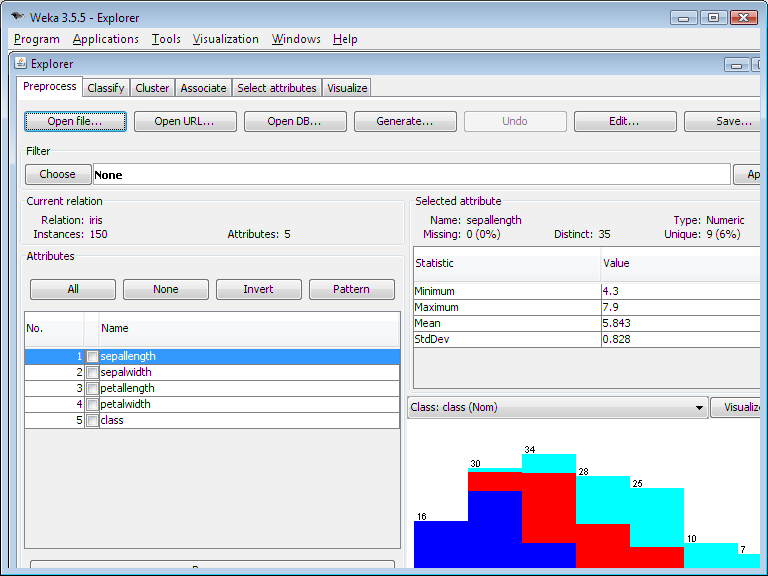
\includegraphics[width=15cm]{pictures/weka.png}
  \caption{Datový soubor otevřený v uživatelském rozhraní Weka}
  \label{fig:weka}
\end{figure}

\textbf{Encog}

Encog je framework pro strojové učení (\textit{Machine Learning}), což je oblast která studuje algoritmy umožňující strojům "učit se". Je to vlastně podoblast umělé inteligence (\textit{Artificial Intelligence}), kterou používají pro studování inteligentního chování, adaptaci ve strojích, a taky pro řízení, rozhodování a plánování procesů v různých systémech.

Tento framework má hodně technik zahrňujících regresní modely, které jsem pravě potřeboval. Komplikace jeho využití byla v tom, že zaklád tohoto frameworku je vytvořen za použití neuronových sítí. Jak jsem zjistil později naučení těchto technologií je časově náročné. Kvůli tomu jsem se rozhodl nechat tento nápad realizace programu a hledat jiné řešení. 


\newpage
\section{Implementace}
\subsection{Datová vrstva}
Jako prvek dat, se kterými pracují výpočetní servery, dostal jsem od svého vedoucího \textit{log file} (nebo taky \textit{žurnál}). Log je to většinou textový soubor s příponou \textit{.log}, který obsahuje záznam činností nějakého programu nebo procesu. Tento záznam je ve tvaru posloupnosti jednotlivých kroků přislušného běhu programu, tj. skládá se z informace o tom jak, kdy, čím nebo kým byla využívána konkretní aplikace, jaké zatížení bylo vyvoláno nebo kolik času trvalo aby se příslušná aplikace proběhla. Používájí se logy pro kontrolu procesů a zjištění přesné příčiny nějaké chyby, pokud k takové došlo. Z jejich záznamů je možno určit co přivedlo k chybě, jaký měla vliv tato chyba a jaké pak měl běžící proces důsledky. 

Daný soubor skládá se z dostatečně velkého množství řádků, v každém ze kterých zaznamenávano několik parametrů. Tyto parametry obsahují svou hodnotu a/nebo svůj název. 

\begin{figure}[h]
  \centering
  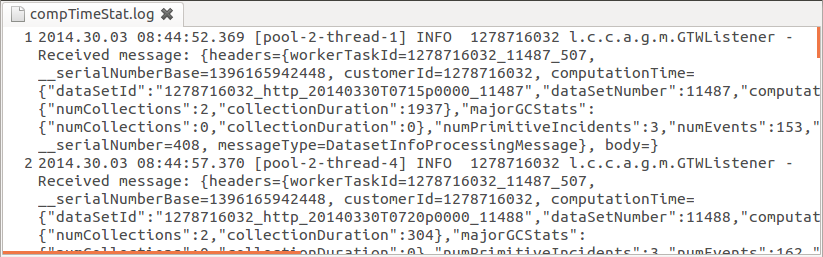
\includegraphics[width=15cm]{pictures/log.png}
  \caption{Log soubor (fragment)}
  \label{fig:log}
\end{figure}

Pro pohodlnější práci se souborem a odstranění nepotřebných parametrů (např. čas, datum) rozhodl jsem se překonvertovat log soubor do souborového formatu \textit{CSV} 	(z angl. \textit{comma-separated values}, nebo hodnoty oddělené čárkami). Je to jeden z nejednoduších formatů pro práci s tabulkovými daty. Považuji vybraný format za vhodný, protože má podobnou strukturu jako u log souboru a je velice používán pro výměnu informací mezi různými systémy. Také dost důležité je, že se sloupce CSV souboru můžou tvářit jako časové řady, které se hodně využívají v regresní analýze.   

\begin{figure}[h]
  \centering
  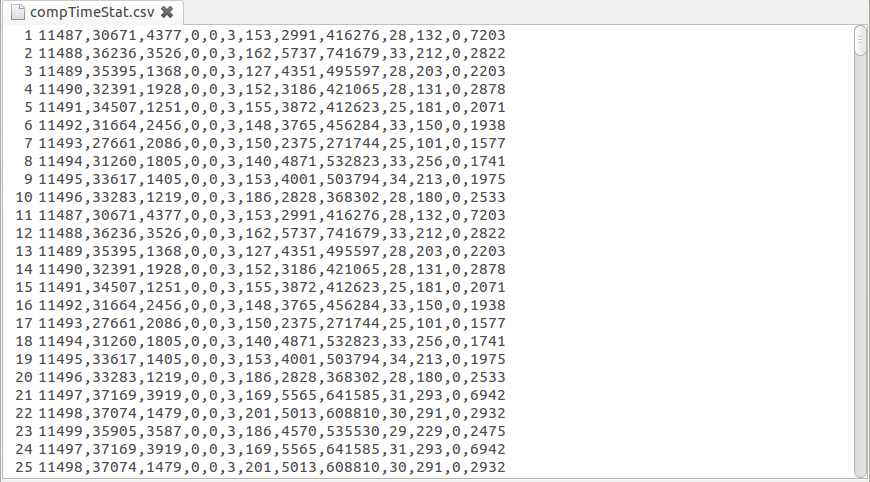
\includegraphics[width=15cm]{pictures/csv.png}
  \caption{CSV soubor (fragment)}
  \label{fig:csv}
\end{figure}

\subsection{Aplikační vrstva}
\subsection{Prezentační vrstva}

\section{Testování aplikace}
\subsection{Testovací data}
\subsection{Zpracování a analýza dat}
\subsection{Predikce}
\subsection{Vizualizace}


\chapter*{Závěr}
\addcontentsline{toc}{chapter}{Závěr} % SEM NESAHEJTE!
%
% Sem napiště závěr
%


\clearpage
\addcontentsline{toc}{chapter}{Literatura} % SEM NESAHEJTE!
\begin{thebibliography}{99}   
	\bibitem FFumio Hayashi. \emph{Econometrics}. Princeton. Princeton University Press. 2000.
	\bibitem TTomáš Cipra. \emph{Analýza časových řad s aplikacemi v ekonomii}. Praha. SNTL - Nakladatelství technické literatury. 1986.
	\bibitem PPetr Fiala. \emph{Úvod do ekonometrie}. Praha. Nakladatelství ČVUT. 2008.
\end{thebibliography}

\newpage % SEM NESAHEJTE!
\addcontentsline{toc}{chapter}{Přílohy} % SEM NESAHEJTE!
\appendix % SEM NESAHEJTE!

\chapter{Název přílohy} % SEM NESAHEJTE!
%
% Zde uveďte seznam příloh
%


\end{document} % SEM NESAHEJTE!
